% Options for packages loaded elsewhere
\PassOptionsToPackage{unicode}{hyperref}
\PassOptionsToPackage{hyphens}{url}
\PassOptionsToPackage{dvipsnames,svgnames,x11names}{xcolor}
%
\documentclass[
  letterpaper,
  DIV=11,
  numbers=noendperiod]{scrreprt}

\usepackage{amsmath,amssymb}
\usepackage{lmodern}
\usepackage{iftex}
\ifPDFTeX
  \usepackage[T1]{fontenc}
  \usepackage[utf8]{inputenc}
  \usepackage{textcomp} % provide euro and other symbols
\else % if luatex or xetex
  \usepackage{unicode-math}
  \defaultfontfeatures{Scale=MatchLowercase}
  \defaultfontfeatures[\rmfamily]{Ligatures=TeX,Scale=1}
\fi
% Use upquote if available, for straight quotes in verbatim environments
\IfFileExists{upquote.sty}{\usepackage{upquote}}{}
\IfFileExists{microtype.sty}{% use microtype if available
  \usepackage[]{microtype}
  \UseMicrotypeSet[protrusion]{basicmath} % disable protrusion for tt fonts
}{}
\makeatletter
\@ifundefined{KOMAClassName}{% if non-KOMA class
  \IfFileExists{parskip.sty}{%
    \usepackage{parskip}
  }{% else
    \setlength{\parindent}{0pt}
    \setlength{\parskip}{6pt plus 2pt minus 1pt}}
}{% if KOMA class
  \KOMAoptions{parskip=half}}
\makeatother
\usepackage{xcolor}
\setlength{\emergencystretch}{3em} % prevent overfull lines
\setcounter{secnumdepth}{5}
% Make \paragraph and \subparagraph free-standing
\ifx\paragraph\undefined\else
  \let\oldparagraph\paragraph
  \renewcommand{\paragraph}[1]{\oldparagraph{#1}\mbox{}}
\fi
\ifx\subparagraph\undefined\else
  \let\oldsubparagraph\subparagraph
  \renewcommand{\subparagraph}[1]{\oldsubparagraph{#1}\mbox{}}
\fi


\providecommand{\tightlist}{%
  \setlength{\itemsep}{0pt}\setlength{\parskip}{0pt}}\usepackage{longtable,booktabs,array}
\usepackage{calc} % for calculating minipage widths
% Correct order of tables after \paragraph or \subparagraph
\usepackage{etoolbox}
\makeatletter
\patchcmd\longtable{\par}{\if@noskipsec\mbox{}\fi\par}{}{}
\makeatother
% Allow footnotes in longtable head/foot
\IfFileExists{footnotehyper.sty}{\usepackage{footnotehyper}}{\usepackage{footnote}}
\makesavenoteenv{longtable}
\usepackage{graphicx}
\makeatletter
\def\maxwidth{\ifdim\Gin@nat@width>\linewidth\linewidth\else\Gin@nat@width\fi}
\def\maxheight{\ifdim\Gin@nat@height>\textheight\textheight\else\Gin@nat@height\fi}
\makeatother
% Scale images if necessary, so that they will not overflow the page
% margins by default, and it is still possible to overwrite the defaults
% using explicit options in \includegraphics[width, height, ...]{}
\setkeys{Gin}{width=\maxwidth,height=\maxheight,keepaspectratio}
% Set default figure placement to htbp
\makeatletter
\def\fps@figure{htbp}
\makeatother
\newlength{\cslhangindent}
\setlength{\cslhangindent}{1.5em}
\newlength{\csllabelwidth}
\setlength{\csllabelwidth}{3em}
\newlength{\cslentryspacingunit} % times entry-spacing
\setlength{\cslentryspacingunit}{\parskip}
\newenvironment{CSLReferences}[2] % #1 hanging-ident, #2 entry spacing
 {% don't indent paragraphs
  \setlength{\parindent}{0pt}
  % turn on hanging indent if param 1 is 1
  \ifodd #1
  \let\oldpar\par
  \def\par{\hangindent=\cslhangindent\oldpar}
  \fi
  % set entry spacing
  \setlength{\parskip}{#2\cslentryspacingunit}
 }%
 {}
\usepackage{calc}
\newcommand{\CSLBlock}[1]{#1\hfill\break}
\newcommand{\CSLLeftMargin}[1]{\parbox[t]{\csllabelwidth}{#1}}
\newcommand{\CSLRightInline}[1]{\parbox[t]{\linewidth - \csllabelwidth}{#1}\break}
\newcommand{\CSLIndent}[1]{\hspace{\cslhangindent}#1}

\KOMAoption{captions}{tableheading}
\makeatletter
\@ifpackageloaded{tcolorbox}{}{\usepackage[many]{tcolorbox}}
\@ifpackageloaded{fontawesome5}{}{\usepackage{fontawesome5}}
\definecolor{quarto-callout-color}{HTML}{909090}
\definecolor{quarto-callout-note-color}{HTML}{0758E5}
\definecolor{quarto-callout-important-color}{HTML}{CC1914}
\definecolor{quarto-callout-warning-color}{HTML}{EB9113}
\definecolor{quarto-callout-tip-color}{HTML}{00A047}
\definecolor{quarto-callout-caution-color}{HTML}{FC5300}
\definecolor{quarto-callout-color-frame}{HTML}{acacac}
\definecolor{quarto-callout-note-color-frame}{HTML}{4582ec}
\definecolor{quarto-callout-important-color-frame}{HTML}{d9534f}
\definecolor{quarto-callout-warning-color-frame}{HTML}{f0ad4e}
\definecolor{quarto-callout-tip-color-frame}{HTML}{02b875}
\definecolor{quarto-callout-caution-color-frame}{HTML}{fd7e14}
\makeatother
\makeatletter
\makeatother
\makeatletter
\@ifpackageloaded{bookmark}{}{\usepackage{bookmark}}
\makeatother
\makeatletter
\@ifpackageloaded{caption}{}{\usepackage{caption}}
\AtBeginDocument{%
\ifdefined\contentsname
  \renewcommand*\contentsname{Table of contents}
\else
  \newcommand\contentsname{Table of contents}
\fi
\ifdefined\listfigurename
  \renewcommand*\listfigurename{List of Figures}
\else
  \newcommand\listfigurename{List of Figures}
\fi
\ifdefined\listtablename
  \renewcommand*\listtablename{List of Tables}
\else
  \newcommand\listtablename{List of Tables}
\fi
\ifdefined\figurename
  \renewcommand*\figurename{Figure}
\else
  \newcommand\figurename{Figure}
\fi
\ifdefined\tablename
  \renewcommand*\tablename{Table}
\else
  \newcommand\tablename{Table}
\fi
}
\@ifpackageloaded{float}{}{\usepackage{float}}
\floatstyle{ruled}
\@ifundefined{c@chapter}{\newfloat{codelisting}{h}{lop}}{\newfloat{codelisting}{h}{lop}[chapter]}
\floatname{codelisting}{Listing}
\newcommand*\listoflistings{\listof{codelisting}{List of Listings}}
\makeatother
\makeatletter
\@ifpackageloaded{caption}{}{\usepackage{caption}}
\@ifpackageloaded{subcaption}{}{\usepackage{subcaption}}
\makeatother
\makeatletter
\@ifpackageloaded{tcolorbox}{}{\usepackage[many]{tcolorbox}}
\makeatother
\makeatletter
\@ifundefined{shadecolor}{\definecolor{shadecolor}{rgb}{.97, .97, .97}}
\makeatother
\makeatletter
\makeatother
\ifLuaTeX
  \usepackage{selnolig}  % disable illegal ligatures
\fi
\IfFileExists{bookmark.sty}{\usepackage{bookmark}}{\usepackage{hyperref}}
\IfFileExists{xurl.sty}{\usepackage{xurl}}{} % add URL line breaks if available
\urlstyle{same} % disable monospaced font for URLs
\hypersetup{
  pdftitle={Physics Text},
  pdfauthor={Jane Doe},
  colorlinks=true,
  linkcolor={blue},
  filecolor={Maroon},
  citecolor={Blue},
  urlcolor={Blue},
  pdfcreator={LaTeX via pandoc}}

\title{Physics Text}
\author{Jane Doe}
\date{3/2/23}

\begin{document}
\maketitle
\ifdefined\Shaded\renewenvironment{Shaded}{\begin{tcolorbox}[interior hidden, boxrule=0pt, frame hidden, borderline west={3pt}{0pt}{shadecolor}, breakable, enhanced, sharp corners]}{\end{tcolorbox}}\fi

\renewcommand*\contentsname{Table of contents}
{
\hypersetup{linkcolor=}
\setcounter{tocdepth}{2}
\tableofcontents
}
\bookmarksetup{startatroot}

\hypertarget{preface}{%
\chapter*{Preface}\label{preface}}
\addcontentsline{toc}{chapter}{Preface}

\markboth{Preface}{Preface}

この本は物理初習者のためのものである.至らぬことも多いかも知れないが,アップデートによって更新していくつもりである.

\bookmarksetup{startatroot}

\hypertarget{ux6570ux5b66ux7684ux6e96ux5099}{%
\chapter{数学的準備}\label{ux6570ux5b66ux7684ux6e96ux5099}}

\hypertarget{ux524dux8aac}{%
\section{前説}\label{ux524dux8aac}}

この章では物理の世界に入る前に知っておかなければならないことを説明します.
\(\require{physics}\)

物理学を始める際にして、初学者の方にはどうしてもある程度の数学の素養が求められます。物理学の発展と数学は決して離すことのできない物であり、例えばみなさんがこれかあら学ぶ力学の分野は、微分と積分の関係性を発見し、それを基礎にしてニュートンが発展させた分野です。
ですがそこが最大の関門として高校生の皆様には立ちはだかることになると思います.ベクトルも微分も積分も,なんなら三角関数もまともにやったことがないのに,いきなり全部を使いこなせることを要求されてしまうからです.
なので,この章では読者が高校1年生の途中くらいから読み始めているものだと想定して,数学について少しずつ勉強を進めながら,物理を始められるところまでやっていこうと思います.関数の定義や三角関数については流石にもう慣れてきたのではないかという時期ですね.もしもまだそこがあやふやであるのならば,まずは数学Iの教科書をある程度進ませてからこの本を読んでいただければ幸いと思っています.
ですが,すでに一通り数学をやっている方ならば,この章を飛ばしていただいても構いません.そのための指標として,まずはこの章におけるゴールを一通り書いておきます.次の表に載せてあることを理解できるようになれば,ひとまずこの章は学び終えたという判定で考えてもらって構いません.

\begin{tcolorbox}[enhanced jigsaw, colbacktitle=quarto-callout-note-color!10!white, opacitybacktitle=0.6, breakable, opacityback=0, titlerule=0mm, leftrule=.75mm, arc=.35mm, colback=white, bottomrule=.15mm, toprule=.15mm, rightrule=.15mm, coltitle=black, left=2mm, colframe=quarto-callout-note-color-frame, toptitle=1mm, title={数学の公式}, bottomtitle=1mm]

\begin{longtable}[]{@{}
  >{\raggedright\arraybackslash}p{(\columnwidth - 2\tabcolsep) * \real{0.2500}}
  >{\raggedright\arraybackslash}p{(\columnwidth - 2\tabcolsep) * \real{0.7500}}@{}}
\toprule()
\endhead
微分の定義 &
\(\dv{x} f(x)=\lim_{\Delta x\rightarrow 0}\frac{f(x+\Delta x)-f(x)}{\Delta x}\) \\
積の微分法 & \(\dv{x}\{f(x)g(x)\}=f'(x)g(x)+f(x)g'(x)\) \\
商の微分法 &
\(\dv{x}\{\frac{f(x)}{g(x)}\}=\frac{f'(x)g(x)-f(x)g'(x)}{\{g(x)\}^2}\) \\
冪函数の微分法 & \(\dv{x}x^r=rx^{r-1}\) \\
\bottomrule()
\end{longtable}

\end{tcolorbox}

では,始めましょう.

\hypertarget{ux6975ux9650}{%
\section{極限}\label{ux6975ux9650}}

関数 \(f(x)=\frac{1}{x}\) を考えます.分母の値である \(x\) が
\(1,10,100,...\) と大きくなるにつれて,関数の値は \(1,0.1,0.01,...\)
と小さくなっていきますね.このような状態のことを次のように書く記すことにします.

\[x \to \infty \; \text{のとき,} \frac{1}{x} \to 0\]

または,

\[ \lim_{x\to\infty}\frac{1}{x}=0\]

この本では後者の方にまとめて書くことにします.
また同様にして,分母の値である \(x\) が \(-1,-10,-100,...\)
と大きくなるにつれて,関数の値は \(-1,-0.1,-0.01,...\) と \(0\)
に近づくことが確認されます.このような状態も次のように書く記すことにします.

\[ \lim_{x\to-\infty}\frac{1}{x}=0\]

次に,分母の値である \(x\) が \(1,0.1,0.01,...\)
と正の値を保ちつつ小さくなる( \(0\) に近づく)につれて,関数の値は
\(1,10,100,...\)
と限りなく大きくなることが確認できます.このような状態も次のように書く記すことにします.

\[ \lim_{x\to +0}\frac{1}{x}=\infty\]

最後に分母の値である \(x\) が \(-1,-0.1,-0.01,...\)
と負の値を保ちつつ小さくなるにつれて,関数の値は \(-1,-10,-100,...\)
と限りなく小さくなることが確認できます.このような状態も次のように書く記すことにします.

\[ \lim_{x\to -0}\frac{1}{x}=-\infty\]

以上の話をまとめると次のようになります.

\begin{tcolorbox}[enhanced jigsaw, colbacktitle=quarto-callout-note-color!10!white, opacitybacktitle=0.6, breakable, opacityback=0, titlerule=0mm, leftrule=.75mm, arc=.35mm, colback=white, bottomrule=.15mm, toprule=.15mm, rightrule=.15mm, coltitle=black, left=2mm, colframe=quarto-callout-note-color-frame, toptitle=1mm, title={定理}, bottomtitle=1mm]

分数の分子が \(0\) でない定数の時,分母の絶対値が大きくなると分数の値は
\(0\) に限りなく近づき,分母が \(0\)
に近づくと分数の絶対値はに限りなく大きくなる.

\end{tcolorbox}

この定理の前半を証明するには \(\frac{c}{x}\)
についてどんなに小さな正の数 \(h\) が指定されようとも,
\(|\frac{c}{x}|<h\) となる \(x\) が存在することを示せば良いです.例えば
\(|x|>\frac{|c|}{h}+1\)
などが存在します.後半については,\(\frac{c}{x}\)
についてどんなに大きな正の数 \(G\) が指定されようとも,
\(|\frac{c}{x}| > G\) となる \(x\)
が存在することを示せば良いです.例えば \(0<|x|<\frac{|c|}{G}\) を満たす
\(x\) などが存在します.

\hypertarget{ux53ceux675f}{%
\section{収束}\label{ux53ceux675f}}

次に,大事な事項である収束について説明します.
まず,次のような関数を考えましょう.

\[f(x) = \frac{x^2-1}{x-1}\]

この関数は \(x=1\) では定義されません.なぜなら,分母が \(0\)
になってしまうからです.では,この関数の \(x=1\)
周辺での様子はどうなっているのでしょうか.周辺なので, \(x\neq 1\)
とすることができます.なので,その時に限り,

\[f(x) = \frac{x^2-1}{x-1}=\frac{(x+1)(x-1)}{x-1}=x+1\]

と式変形することができ, \(x+1\) の値は \(x\) が限りなく \(1\)
に近づく際には, \(2\)
に限りなく近づくことになります.この状態のことを次のように書き表します.

\[ \lim_{x\to 1}f(x)=2\]

このことをまとめ上げると次のようになります.

\begin{tcolorbox}[enhanced jigsaw, colbacktitle=quarto-callout-note-color!10!white, opacitybacktitle=0.6, breakable, opacityback=0, titlerule=0mm, leftrule=.75mm, arc=.35mm, colback=white, bottomrule=.15mm, toprule=.15mm, rightrule=.15mm, coltitle=black, left=2mm, colframe=quarto-callout-note-color-frame, toptitle=1mm, title={定義}, bottomtitle=1mm]

\(f(x)\) が \(x=a\) の近くで定義されている関数で, \(x\) が \(a\)
に近づく時,\(f(x)\) が限りなく \(\alpha\) に近づく時,次のように書く.

\[ \lim_{x\to a}f(x)=\alpha\]

ただし, \(f(x)\) は \(x=a\) において定義されていなくとも良い.また,
\(x\) が \(a\) より大きな値から \(a\) に近づくときは \(\lim_{x\to a+0}\)
と書き,\(x\) が \(a\) より小さな値から \(a\) に近づくときは
\(\lim_{x\to a-0}\) と書く.

\end{tcolorbox}

以上の知識を持って,実際に問題を解いてみましょう.

\begin{tcolorbox}[enhanced jigsaw, colbacktitle=quarto-callout-tip-color!10!white, opacitybacktitle=0.6, breakable, opacityback=0, titlerule=0mm, leftrule=.75mm, arc=.35mm, colback=white, bottomrule=.15mm, toprule=.15mm, rightrule=.15mm, coltitle=black, left=2mm, colframe=quarto-callout-tip-color-frame, toptitle=1mm, title={問題}, bottomtitle=1mm]

\begin{longtable}[]{@{}
  >{\raggedright\arraybackslash}p{(\columnwidth - 2\tabcolsep) * \real{0.5000}}
  >{\raggedright\arraybackslash}p{(\columnwidth - 2\tabcolsep) * \real{0.5000}}@{}}
\toprule()
\endhead
\(\lim_{x\to 1}\frac{x^2-x}{x^2+x-2}\) &
\(\lim_{x\to 2}\frac{x-2}{\sqrt{x}-\sqrt{2}}\) \\
\(\lim_{x\to 1}\frac{2-\sqrt{a-x}}{1-x}=b\;\text{収束する}\) &
\(\lim_{x\to -\infty}x(\sqrt{x^2-2x+3}+x-a)\;\text{収束する}\) \\
\bottomrule()
\end{longtable}

\end{tcolorbox}

解答

\begin{longtable}[]{@{}ll@{}}
\toprule()
\endhead
\(\frac{1}{3}\) & \(2\sqrt{2}\) \\
\(a=5,\;b=-\frac{1}{4}\) & \(a=1,\;b=-1\) \\
\bottomrule()
\end{longtable}

\begin{tcolorbox}[enhanced jigsaw, colbacktitle=quarto-callout-tip-color!10!white, opacitybacktitle=0.6, breakable, opacityback=0, titlerule=0mm, leftrule=.75mm, arc=.35mm, colback=white, bottomrule=.15mm, toprule=.15mm, rightrule=.15mm, coltitle=black, left=2mm, colframe=quarto-callout-tip-color-frame, toptitle=1mm, title={問題}, bottomtitle=1mm]

\[f(x)=\frac{2ax^2-(a-2)x-1}{ax^2-(a^2-1)x-a}\]
と定義された関数があり,次の式が成り立つように \(a\) の値を定めよ.
\[\lim_{x \to 1}f(x)=\frac{1}{2}\]

\end{tcolorbox}

解答

\[f(x)=\frac{(2x-1)(ax+1)}{(x-a)(ax+1)}=\frac{2x-1}{x-a}\]
となっているので,極限を計算すると \[\frac{1}{1-a}=\frac{1}{2}\]
\[a=-1\]

とわかる.

\hypertarget{ux5546ux5faeux5206}{%
\section{商微分}\label{ux5546ux5faeux5206}}

ある関数 \(f(x)\)
を考えてみることにしましょう.この関数の振る舞いを考える際には定義式自体の形を見て,対称性や式変形などを駆使することが多いと思われます.ここではその振る舞いを考える方法の一つを紹介してみたいと思います.

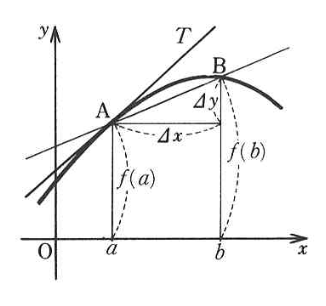
\includegraphics{./images/intro-1.png}

上の図のように, \(f(x)\) が \(x=a\) から \(x=b=a+\Delta x\)
だけ変化して場合に, \(\Delta y\)
だけの変化が起きるものとします.\(\Delta x,\; \Delta y\)
は一つの変数であり,増分と呼ばれます.
その時次の式が成り立つかと思われます.

\[\Delta y = \frac{f(b)-f(a)}{b-a} \Delta x\]

この式を次のように変形することによって,この式の概要が見やすくなるでしょう.

\[ f(b) = f(a) + \frac{\Delta y}{\Delta x}(b-a) \]

この式が表すものとは, \(f(b)\) の値が \(f(a)\) の値から
\(\frac{\Delta y}{\Delta x}(b-a)=\text{ABの傾き}\times a\text{と}b\text{の違いの分}\)
だけずれているということになるわけです. この時,
\(\frac{\Delta y}{\Delta x}\) の値を \(\Delta x\to 0\)
と極限をとって考えれば,ABの傾きは点Aにおける接線の傾きになるわけです.このとき,次のように書き記すことにします.

\[\lim_{\Delta x \to 0}\frac{\Delta y}{\Delta x}=\dv{y}{x}=y'=f'(x)\]

この値のことを微分係数と呼んでいます.先ほどの式を微分係数を使って書き直してあげれば次のようになるわけです.

\[ f(b) = f(a) + \frac{\Delta y}{\Delta x}(b-a) \]

\[ \Delta y = \dv{y}{x} \Delta x\]

ここで近似値にしたのは, \(\Delta x\)
をしっかりと極限とっていないからですが,今までやってきたことが接線を使って近似をしているというのがわかりやすい形なので採用しました.
この式の言わんとするところは,十分小さな \(\Delta x\) に関して言えば
\(\Delta y\) は接戦の傾きで近似できるということです.

以上のことを実際の具体的な関数でやってみましょう.例えば, \(f(x)=x^2\)
などを考えれば

\[\Delta y = \frac{b^2-a^2}{b-a} \Delta x = (b+a) \Delta x = (2a+\Delta x) \Delta x\]

と式変形がなされるわけです.これによって \(\Delta y,\; \Delta x\)
の比は次のように書き表され

\[\frac{\Delta y}{\Delta x} = 2a + \Delta x\]

となります.そして,極限を取ることによって

\[\dv{y}{x}=2a\]

となります.このことを \(f(x)\) の \(x=a\) における微分係数は \(2a\)
であると呼び,次のように表すことが多いです.

\[ \dv{y}{x}|_{x=a}=f'(a)=2a\]

また, \(a\) という具体的に代入した値ではなく,任意の \(x\)
についても同様なことが言えるため,

\[ \dv{y}{x}=f'(x)=2x\]

と書くことになります.
以上述べたように,微分を考える理由とは,接線で曲線を近似してみようという試みであり,また,曲線を非常に小さな部分で見てあげれば直線になると考えていることになります.

実際に問題を解いてみましょう.

\begin{tcolorbox}[enhanced jigsaw, colbacktitle=quarto-callout-warning-color!10!white, opacitybacktitle=0.6, breakable, opacityback=0, titlerule=0mm, leftrule=.75mm, arc=.35mm, colback=white, bottomrule=.15mm, toprule=.15mm, rightrule=.15mm, coltitle=black, left=2mm, colframe=quarto-callout-warning-color-frame, toptitle=1mm, title={例題}, bottomtitle=1mm]

次の関数の微分係数を求めよ. \[f(x)=x^3+x+1\]

\end{tcolorbox}

解答

\(a=x,\;b=a+\Delta x\) とする.
\[\Delta y = \frac{f(b)-f(a)}{b-a}\Delta x\]
\[\frac{f(b)-f(a)}{b-a}=\frac{f(a+\Delta x)-f(a)}{a+\Delta x -a} \]
\[= \frac{3x^2\Delta x + 3x\Delta x^2 + \Delta x ^3 + \Delta x}{\Delta x}\]
\[=3x^2+ 3x\Delta x + \Delta x ^2 + 1 \to_{\Delta x \to 0} 3x^2+1\]
\[\dv{y}{x}=3x^2+1\]

次に微分係数に慣れてもらうために問題を置いておきます.

\begin{tcolorbox}[enhanced jigsaw, colbacktitle=quarto-callout-tip-color!10!white, opacitybacktitle=0.6, breakable, opacityback=0, titlerule=0mm, leftrule=.75mm, arc=.35mm, colback=white, bottomrule=.15mm, toprule=.15mm, rightrule=.15mm, coltitle=black, left=2mm, colframe=quarto-callout-tip-color-frame, toptitle=1mm, title={例題}, bottomtitle=1mm]

次の関数の微分係数を求めよ. \[f(x)=x^3+x+1\]

\end{tcolorbox}

解答

\(a=x,\;b=a+\Delta x\) とする.
\[\Delta y = \frac{f(b)-f(a)}{b-a}\Delta x\]
\[\frac{f(b)-f(a)}{b-a}=\frac{f(a+\Delta x)-f(a)}{a+\Delta x -a} \]
\[= \frac{3x^2\Delta x + 3x\Delta x^2 + \Delta x ^3 + \Delta x}{\Delta x}\]
\[=3x^2+ 3x\Delta x + \Delta x ^2 + 1 \to_{\Delta x \to 0} 3x^2+1\]
\[\dv{y}{x}=3x^2+1\]

\bookmarksetup{startatroot}

\hypertarget{summary}{%
\chapter{Summary}\label{summary}}

In summary, this book has no content whatsoever.

\bookmarksetup{startatroot}

\hypertarget{references}{%
\chapter*{References}\label{references}}
\addcontentsline{toc}{chapter}{References}

\markboth{References}{References}

\hypertarget{refs}{}
\begin{CSLReferences}{0}{0}
\end{CSLReferences}



\end{document}
